\documentclass[11pt,oneside,a4paper]{article}

\usepackage[utf8]{inputenc} % ci sono delle lettere accentate nelle note
\usepackage{booktabs}
\newcommand{\otoprule}{\midrule[\heavyrulewidth]}
\newcommand{\lmidrule}{\midrule[.5\heavyrulewidth]}
\usepackage{tabularx}
\newcolumntype{W}{>{\centering\arraybackslash}X}
\newcolumntype{C}{>{\centering\arraybackslash}X}
\usepackage{multirow}
\usepackage{textcomp}
\usepackage{xcolor}
\usepackage{authblk}

\usepackage{graphicx}

\usepackage{tikz}
\usetikzlibrary{shapes,arrows}
\usetikzlibrary{decorations,decorations.pathmorphing,decorations.markings}
\usetikzlibrary{positioning,patterns,fit}
\usetikzlibrary{matrix}
\usetikzlibrary{calc}

\newcommand{\parentesi}[6]{%
\coordinate (#6) at ($(#1.north east)!0.5!(#2.south east) + (#3,0pt)$);
\draw[#5] (#1.north east) -| (#6) |- (#2.south east);
\node[right] at (#6) {#4};
}
\colorlet{grig}{gray}
\colorlet{grigl}{gray!60!white}

\tikzset{%
  freccia/.style={->,shorten >=1pt,rounded corners=1pt},
  parentesi/.style={shorten >=1pt,shorten <=1pt,semithick},
  ziged/.style={%
    decorate,
    decoration={zigzag,segment length=3pt,amplitude=0.5pt},
    white
  },
  extlabel/.style={%
    inner sep=0pt, text height=2.5ex,
    minimum height=2.5ex,
    dashed, draw, rounded corners=5pt, thick, font=\footnotesize
  },
  read matrix/.style={%
    matrix of nodes,
    nodes in empty cells,
    text depth=0.3ex,
    text height=1.5ex,
    text width=1.1em,
    nodes={%
      font={\ttfamily},
      minimum height=1.3em,
      align=center
    },
    column 1/.style={%
      nodes={%
        text width=3ex,
        align=left
      }
    }
  }
}

\newcommand{\rot}{\ensuremath{\mathit{RT}}}
\newcommand{\SA}{\ensuremath{\mathit{SA}}}
\newcommand{\LCP}{\ensuremath{\mathit{L}}}


\newcommand{\ie}{\textit{i.e.},\xspace}
\newcommand{\notaestesa}[2]{%
  \marginpar{\color{red!75!black}\textbf{\texttimes}}%
  {\color{red!75!black}%
    [\,\textbullet\,\textsf{\textbf{#1:}} %
    \textsf{\footnotesize#2}\,\textbullet\,]}%
}
\newcommand{\SB}[1]{\notaestesa{SB}{#1}}
\newcommand{\PB}[1]{\notaestesa{PB}{#1}}
\newcommand{\MP}[1]{\notaestesa{MP}{#1}}
\newcommand{\YP}[1]{\notaestesa{YP}{#1}}
\begin{document}

\title{Efficient construction of de Bruijn and string graphs:
an algorithmic view of assembly graphs}

\author[1]{Stefano Beretta}
\author[1]{Marco Previtali}
\author[1]{Raffaella Rizzi}
\author[1]{Yuri Pirola}	
\author[1]{Gianluca Della Vedova}
\author[1]{Paola Bonizzoni}

\affil[1]{Department of Computer Science, Systems and Communications,
University of Milan-Bicocca, Italy}

\date{}

\maketitle

\textbf{Keywords:} de Bruijn graphs;
string graphs;
Burrows-Wheeler Transform;
genome assembly.


\begin{abstract}
De novo assembly of large sequences from sequence reads typically employs
either string or de Bruijn graphs.
%
The former are the basis for most assemblers designed for Sanger sequences,
while the latter have been extensively used in assemblers designed for second
generation sequence data.

Contemporary, sequencing platforms can produce terabytes of data and the
construction and navigation of assembly graphs pose significant computational
challenges.
%
In particular, the generation and maintenance of compact representations of
such graphs must attain a satisfactory balance of main memory usage and runtime.
%
Since these challenges are becoming more critical as ever larger datasets are
produced, several promising approaches to graph construction and storage have
been proposed and implemented.

In this review, we discuss both the use of the Burrows-Wheeler Transform and the FM-index in the construction and representation of de Bruijn and string graphs, and the incorporation of other computational techniques, such as the Bloom filter, to allow compact representation of such graphs.
%
We show, with quantified examples, that by working on compact, yet functionally complete, representations of the input data, great savings in memory usage can be obtained with negligible increases in run times.
\end{abstract}

\section{Introduction}
The widespread adoption of Next-Generation Sequencing (NGS) technologies,
and the associated increase in production of sequence data, has revitalized
algorithmic research, particularly with respect to de novo sequence
assembly --- still a partially unsolved problem for large and complex genomes.

De novo assembly pipelines, for genomes, metagenomes or transcriptomes, can
generally be divided into three main phases.
%
First, raw sequence data are subjected to quality checks, trimming/merging of
paired ends, and probabilistic error correction.
%
Secondly, contigs (stretches of contiguous sequences composed of overlapping
reads) are generated.
%
Finally, linked, but non-overlapping contigs are united in scaffolds using
information from paired ends or other sources.
%
While all these steps are critical to the generation of reliable assemblies,
the current review focuses on algorithmic aspects related to the construction
and storage of data structures needed in the contig generation step.
%
We direct the interested readers
to~\cite{Yang2013, Laehnemann2016, Hunt2014} for recent discussions of data
pre-processing and scaffolding approaches. 

Graph representations of relationships between common portions of the reads
are fundamental to contig generation.
%
Early assemblers, designed specifically for Sanger reads, typically employ string
graphs~\cite{Myers2005} --- where vertices represent reads and edges correspond
to overlaps --- while assemblers designed for short read data often employ
de Bruijn graphs (dBGs)~\cite{compeau2011} --- where vertices represent $k$-mers
(substrings of length $k$ of some reads) and each edge connects two $k$-mers
having an overlap of length $k-1$.
%
String graphs are more informative (with respect to relationships between input
reads) than dBGs but they are computationally more expensive to produce,
especially where datasets contain hundreds of millions of reads, since all
pairs of reads should be compared.

Both representations share the concept that an assembly corresponds to a path
in the graph, and, under ideal conditions (including the absence of sequence
errors, repeats, and heterozygosity), it should be possible to reconstruct only
one relevant path for each genomic replicon corresponding to the correct assembly.
%
Unfortunately, sequencing errors occur frequently in NGS data, while repeats and
heterozygosity are common in genomic DNA, and transcriptomic or metagenomic data
show some peculiarities (such as alternative splicing and RNA editing for the
former and variable levels of represented transcripts/genomes in both cases)
which require the incorporation of various assumptions into specialized assemblers
to facilitate graph traversal and contig generation.
%
Nevertheless, the initial construction and storage of assembly graphs from input
sequence data are steps shared by almost all current assemblers, and typically
represent the most computationally intensive steps in sequence assembly.

Here, we present commonalities and differences among assembly approaches based
on string graphs and dBGs, emphasizing recent research efforts to address the
scalability issues that arise when dealing with huge collections of reads derived
from complex and sometimes repeat-rich or heterozygous templates.
%
% In particular, we present the use of compressed data structures to index huge collections of reads and quickly perform substring operations such as recovering Longest Common Prefix arrays~\cite{Abouelhoda2004} and maximal overlaps between reads.
%
Furthermore, we discuss the significance of external memory
algorithms~\cite{DBLP:conf/wabi/BonizzoniVPPR14} in the trade-off between
execution times and memory requirements, and the use of the Bloom filter in
compacting graph representations.

The rest of the review is organized as follows.
%
In Section~\ref{sec:string-graph} we consider sequence assembly by the Overlap
Layout Consensus approach using string graphs and the incorporation of
computationally efficient data structures, such as the Burrows-Wheeler Transform
(BWT)~\cite{Burrows1994} and the FM-index~\cite{Ferragina2005}  --- providing
an experimental comparison of the space and time efficiency for alternative
graph construction strategies.
%
Section~\ref{sec:DBG} is devoted to the presentation of recent advances in dBG
construction and representation with membership and navigational data structures.
%
Again, the space and time efficiency of such assemblers is compared, and improvements in data representation are quantified.
%
Finally, we conclude the paper (Section~\ref{sec:conclusions}) posing some open problems.

\section{String graphs in the Overlap Layout Consensus}
\label{sec:string-graph}

% The Overlap Layout Consensus (OLC) is a class of algorithms to assemble sequences from a set of reads, wherein overlap graphs ---  where vertices are the input reads and edges link overlapping reads. Here, assembly consists of three steps: (i) building the
The Overlap Layout Consensus (OLC) is a class of algorithms to assemble sequences from a set of reads, that generally consists of three steps: (i) building the
 \emph{overlap graph} from the set of reads, (ii) reducing the
overlap graph to the \emph{string graph} (the assembly graph) by removing redundant edges (not helpful in assembling the genome), and (iii)
determining the genome sequence by traversing 
the string graph. Given a set $R$ of strings (\textit{i.e.}, the reads), the \emph{overlap graph} is the directed graph whose vertices are the strings in
$R$, and an edge $(r_i,r_j)$ from string $r_i$ to string $r_j$ exists if
a suffix of $r_i$ is equal to a prefix of $r_j$, that is if they
\emph{overlap}.
A path in the overlap graph (or in the string graph) represents a string that is obtained by assembling the reads along the path.
% The suffix of $r_j$ (or the prefix of $r_i$) exceeding the overlap is usually used as the \emph{label} of the edge $(r_i,r_j)$.
An edge $(r_i,r_j)$ is reducible (or redundant) if a path from $r_i$ to $r_j$ including another vertex but representing the same string of $(r_i,r_j)$ exists.
% Reducible edges are not useful in the generation of unambiguous assemblies, so they can be removed from the overlap graph, resulting in the string graph.
As a consequence, reducible edges can be removed from the overlap graph without affecting the resulting assemblies.
The string graph is defined as the result of this removal process and, since it can be significantly smaller than the overlap graph, it is the graph representation generally traversed to generate the final contigs.

Both overlap and string graphs were initially proposed in~\cite{Myers2005} and have been incorporated into numerous assembly programs for Sanger reads.
A practical advantage of overlap/string graphs over dBGs is that they can immediately disambiguate short repeats that dBGs might resolve only at later stages.
% However, the computation of the overlap graph is time and space consuming and is the bottleneck of OLC pipelines, particularly in the analyses of NGS data~\cite{readjoiner}. 
However, the computation of overlap/string graphs is time and space consuming and is the bottleneck of OLC pipelines.
% particularly in the analyses of NGS data~\cite{readjoiner}. 
In particular, it was unpractical for the analyses of NGS data until the first algorithms using efficient indexing data structures (such as the Burrows-Wheeler Transform and the FM-index) were proposed~\cite{Simpson2012}.

% \subsection{String graphs and indexing data structures}
% String graph assemblers rely on efficient indexing data structures
% to detect the overlaps between reads. Indeed, both overlaps between input reads and, especially, string graphs are computationally intensive to construct~\cite{Simpson2012}.

The Burrows-Wheeler Transform (BWT), which is employed by many tools that align NGS reads to reference sequences~\cite{Li15072009,Langmead2009}, as well as the related FM-index provide succinct and lossless data representations~\cite{cox_large-scale_2012}.
The BWT~\cite{Burrows1994} of a set $R$ of reads is
a permutation $B$ of their symbols such that $B[i]$ is the symbol preceding the
$i$-th smallest element in the lexicographic ordered set of all suffixes of the
reads in $R$.
A sentinel symbol $\$$, that lexicographically precedes all symbols in
the alphabet of the reads, is appended to each read in order to disambiguate two identical suffixes.


\begin{figure}[t]
\centering
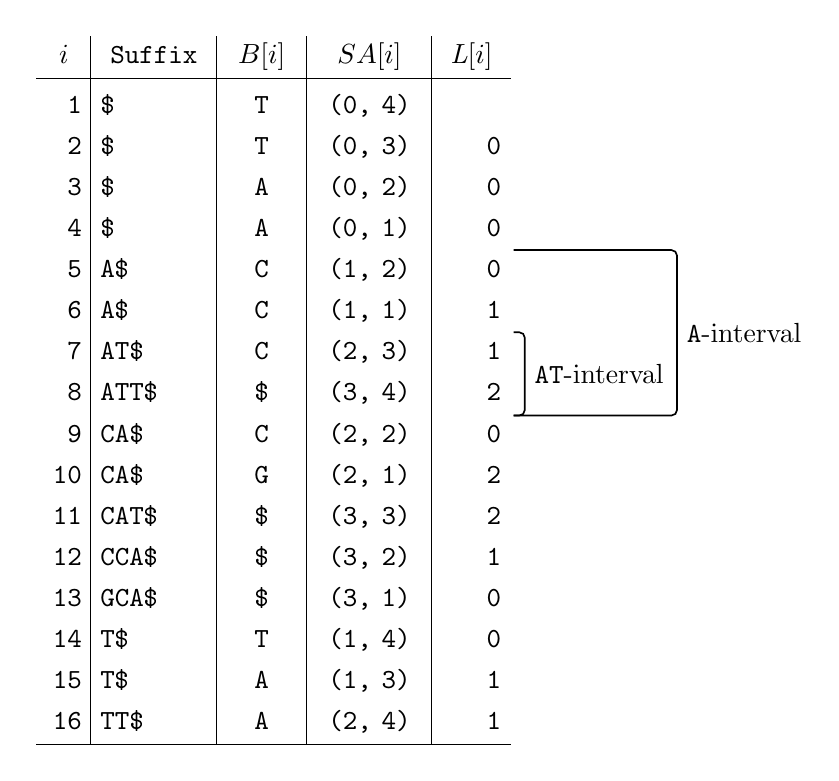
\begin{tikzpicture}
\matrix (m) [matrix of nodes,
nodes in empty cells,
text depth=0.4ex,text height=1.5ex,
nodes={font={\ttfamily},minimum height=1.3em},
column sep=0,row sep=0,
column 1/.style={nodes={text width=3ex, align=right}},
column 2/.style={nodes={text width=9ex, align=left}},
column 3/.style={nodes={text width=6ex, align=center}},
column 4/.style={nodes={text width=9ex, align=center}},
column 5/.style={nodes={text width=5ex, align=right}},
row 1/.style={nodes={align=center}}
]{
$i$ & Suffix & $B[i]$ & $SA[i]$ & $\LCP[i]$ \\[3pt]
1  & \$\color{grig}          &    T     & (0, 4) & \\
2  & \$\color{grig}          &    T     & (0, 3) & 0 \\
3  & \$\color{grig}          &    A     & (0, 2) & 0 \\
4  & \$\color{grig}          &    A     & (0, 1) & 0 \\
5  & A\$\color{grig}          &    C     & (1, 2) & 0 \\
6  & A\$\color{grig}          &    C     & (1, 1) & 1 \\
7  & AT\$\color{grig}          &    C     & (2, 3) & 1 \\
8  & ATT\$                     &    \$    & (3, 4) & 2 \\
9  & CA\$\color{grig}          &    C     & (2, 2) & 0 \\
10 & CA\$\color{grig}         &    G     & (2, 1) & 2 \\
11 & CAT\$                     &    \$    & (3, 3) & 2 \\
12 & CCA\$                     &    \$    & (3, 2) & 1 \\
13 & GCA\$                     &    \$    & (3, 1) & 0 \\
14 & T\$\color{grig}          &    T     & (1, 4) & 0 \\
15 & T\$\color{grig}          &    A     & (1, 3) & 1 \\
16 & TT\$\color{grig}          &    A     & (2, 4) & 1 \\
};

\draw (m-1-1.south west) -- (m-1-5.south east);
\draw (m-17-1.south west) -- (m-17-5.south east);
\foreach \y in {2,3,4,5} {
  \draw (m-1-\y.north west) -- (m-17-\y.south west);
};

\parentesi{m-6-5}{m-9-5}{6em}{$\mathtt{A}$-interval}{parentesi,rounded corners=2pt}{mid1}
\parentesi{m-8-5}{m-9-5}{0.5em}{$\mathtt{AT}$-interval}{parentesi,rounded corners=2pt}{mid2}
\end{tikzpicture}
\caption{Example of BWT, GSA and LCP array of reads $r_1=\mathtt{GCA}$, $r_2=\mathtt{CCA}$, $r_3=\mathtt{CAT}$, and $r_4=\mathtt{ATT}$.
The black portion of the column \emph{Suffix} lists the suffixes in lexicographic order.}
\label{fig:example-bwt}
\end{figure}


Other data structures related to the BWT include: Generalized Suffix Arrays (GSA), Longest Common Prefix (LCP) arrays, and
the FM-index.
The Generalized Suffix Array (GSA)~\cite{Shi1996} of a set $R$ is the array
$\SA$ where the element $\SA[i]$ points to the $i$-th smallest suffix of $R$
in lexicographic order. 
The Longest Common Prefix (LCP) array~\cite{Manber93} is the array $\LCP$ such
that $\LCP[i]$ is equal to the length of the longest prefix shared by the suffixes
pointed by $\SA[i]$ and $\SA[i-1]$.
The $i$-th symbol $B[i]$ of the BWT is the symbol preceding the suffix pointed by 
$\SA[i]$.
All suffixes having a common prefix $Q$ appear consecutively in an interval
$[b,e]$ of $\SA$, which is called \emph{$Q$-interval}. A $Q$-interval represents the occurrences of the string $Q$ in the set $R$.
Since $\SA$ and $B$ are closely related, $[b,e]$ on the BWT $B$ is also called $Q$-interval, and $B[b,e]$ are the symbols preceding the suffixes sharing the common prefix $Q$.

The FM-index~\cite{Ferragina2005} is a self-index relying on the relation between GSA and BWT. It consists of two functions $C$ and
$Occ$, where $C(\sigma)$ is the number of occurrences of symbols that are lexicographically smaller than $\sigma$ in $B$
and
$Occ(\sigma,i)$ is the number of occurrences of $\sigma$ in the prefix of
the first $i-1$ symbols of $B$.
The FM-index allows the efficient backward $\sigma$-extension of the $\sigma Q$-interval related to the suffixes sharing the common prefix $\sigma Q$, and representing the occurrences of the string $\sigma Q$ in the set $R$. Moreover, the FM-index together with the well-known notion of the \emph{bidirectional} BWT~\cite{Lam2009} also allow the forward $\sigma$-extension of the $Q \sigma$-interval related to the suffixes having $Q \sigma$ as a common prefix. These two operations are the basis of pattern matching over the reads in a set $R$:
those ideas lead to linear-time algorithms for pattern matching.
%
Indeed, both backward and forward $\sigma$-extensions need constant time, once the functions $C$
and $Occ$, and the BWT are given. 

Several algorithms to construct the BWT of a large
collection of short reads have been proposed.
Among them, we point out BCR and BCRext~\cite{Bauer2011}, which 
construct the BWT in external memory and are freely available as part of the BEETL suite.
%,
%and both are based on an iterative procedure, where each iteration $j$ computes
%the permutation of the symbols preceding the suffixes of length at most $j$, for increasing values of $j$.
%by simulating the insertion, in the BWT that has been computed at the previous
%iteration, of the suffixes of length exactly equal to $j$.
%
%At each iteration, the partial BWT is partitioned into segments $B_j(\sigma)$
%(which are external files) such that $B_j(\sigma)$ is the BWT segment related to the suffixes
%starting with symbol $\sigma$.
%
%At the end of the iterations, these segments contain the BWT of the input collection.
%
% Both approaches are implemented in the suite BEETL for building and manipulating
% the BWT of a large collection of strings.
%
%Another tool to build the BWT is ropeBWT2~\cite{Li15112014} that is suitable to
%process long reads as well as short reads. 

\subsection{BWT-based  string graph construction}

In this section we present three tools for string graph construction: String Graph Assembler (SGA)~\cite{Simpson2010,Simpson2012}, Light String Graph (LSG)~\cite{Bonizzoni2015}, and Readjoiner~\cite{readjoiner}.
%
Both SGA and LSG employ the BWT and the FM-index, while Readjoiner uses hashing data structures.

\paragraph{}
\textbf{SGA}~\cite{Simpson2010, Simpson2012} constructs the FM-index of the input reads, together with the bidirectional BWT~\cite{Lam2009}, and uses those structures to
efficiently compute the string graph. For each  read $r$ in the input set $R$, all 
suffixes of $r$ are computed by increasing length by performing backward
extensions on the BWT of $R$. Reads that have an overlap $Q$ with $r$ are easily found by detecting the presence of the sentinel symbol in the $Q$-interval of the BWT. SGA considers both possible DNA strands from which reads might derive. The bidirectional BWT is then used to detect and output the irreducible edges of the string graph.
The original version of SGA was estimated to require $700$GB of main memory for indexing a $20x$ coverage human genome dataset~\cite{Simpson2010}.

The SGA pipeline has a preprocessing step for filtering and trimming input
reads with multiple low-quality or ambiguous base calls~\cite{Simpson2012}.
A preliminary FM-index is built to facilitate error correction using $k$-mer frequencies. After graph construction and traversal, contigs are assembled into scaffolds using information from paired-end reads.

SGA can use RopeBWT2~\cite{Li15112014} or SA-IS to index the
input reads. The former, an in-memory
implementation of BCR~\cite{Bauer2011}, works well with short strings ($\leq 200$bp).
SA-IS relies on induced
sorting~\cite{nong_two_2011} to build suffix arrays and is slower but works well for very long sequences.
% * <david.horner@unimi.it> 2016-09-28T12:48:10.907Z:
%
% Guys, I have taken the liberty of removing all reference to and trace of "fermi". There is a discussion of the method (which was designed for a different problem to "true de-novo assembly" and which we neither test nor discuss ANYWHERE else in the paper. IMHO this is a justified cut, however if you feel strongly that it should be mentioned, feel free to re-insert and I will check the English.
%
% ^ <david.horner@unimi.it> 2016-09-28T12:50:51.743Z.
\paragraph{}
\textbf{LSG}~\cite{Bonizzoni2015} is a string graph construction algorithm and requires the BWT of the input reads.
It employs a slightly modified version of BEETL~\cite{Bauer2011} for preliminary read indexing and computes the
GSA, BWT and LCP array of the input reads in external memory, minimizing the amount of data maintained in RAM.
It does not in itself perform graph traversal and contig assembly.

While SGA processes each read to compute the overlaps with other reads,  LSG  employs a single synchronous scan of BWT, GSA and LCP array to compute all overlaps that are at least $l_m$ long
(where $l_m$ is the minimum length of an overlap), and to represent them as $Q$-intervals (that is, BWT intervals).
Subsequently, a sequence of backward extensions from these intervals allows to compute the labels of the edges of the overlap graph (the label is the prefix exceeding the overlap) and, at the same time, record only the non-redundant edges of the string graph. Integration of LSG into the SGA pipeline produces a complete string graph-based assembler whose memory requirements allow to assemble the human genome on a standard workstation.
Some of the ideas presented in LSG have recently been applied to in-memory string graph construction, Fast String Graph~\cite{isbra2016-fsg}, that is faster
than SGA.    

\paragraph{}
\textbf{Readjoiner}~\cite{readjoiner} first identifies and lexicographically sorts all suffixes that are involved in a suffix-prefix match  (SPM-suffixes), i.e.~all read
suffixes that are at least $l_m$ symbols long ($l_m$ is the minimum overlap
length), and share a prefix of length $\geq k$ (where $k \leq l_m$ is a parameter chosen on the basis of a time/space trade-off) with other read(s) in the input set.
Then, from the sorted set of SPM-suffixes, the algorithm computes the
suffix-prefix matches (overlaps) and outputs the irreducible edges of the graph, by subsequent rounds of suffix sorting, scanning, and filtering.

\subsection{Comparing string graph approaches in genome assembly}

We have performed a limited comparison of string graph construction and genome
assembly using data representation approaches discussed in this review.
%
The NA12878 sample of the $1000$ Genomes Project matching read group
``20FUK'', recently used in a published comparison of string graph
assemblers~\cite{Bonizzoni2015}, was downloaded and subjected to the
first five (pre-processing) steps of the workflow used by SGA in the
GAGE competition~\cite{salzberg2012gage} as reported
in~\texttt{http://gage.cbcb.umd.edu/recipes/sga.html}.
%
The resulting filtered dataset contained approximately $875$ million
of $101$bp reads.
%
The main goal of the analysis was to evaluate the effective computational performance of the tools, with respect to the construction of
the string graph --- one of the main steps of the assembly
process --- while verifying that in-memory or disk-located graph
representations had negligible effects on the assembly quality.
%
For all tools, a minimum overlap of $65$bp was required.
%
Tables~\ref{table:full-dataset-total-times}
and~\ref{table:full-dataset-total-quality} in the Supplementary Materials
summarize the results.
%
We first compared LSG~\cite{Bonizzoni2015} and
SGA~\cite{Simpson2010,Simpson2012} by examining the running time and
the memory usage peak of the three-phases genome assembly: (i) indexing,
(ii) string graph construction (including the output of the graph), and
(iii) assembly.
%
It should be recalled that LSG is an external-memory approach while SGA
is in-memory.
%
Since LSG does not perform genome assembly, to allow a direct evaluation
of the impact of graph construction on the genome assembly, the SGA assembly
phase was coupled with the LSG graph construction.
%
The indexing of the input reads was performed with Ropebwt2~\cite{Li15112014}
for SGA, and with BEETL for LSG.
%
Indeed, BEETL was the main bottleneck for LSG, since it used $52$GB of
memory to compute the indexing structures, while SGA required $26$GB of
memory during the indexing phase.
%
This latter step took $9,540$ minutes  for LSG (using BEETL)
and $1,112$ minutes for SGA (using Ropebwt).
%
During the string graph construction phase, SGA and LSG had a memory peak
of $106$GB and $46$GB, respectively.
%
The memory used to compute the string graph (excluding the output) was
$43$GB and $0.87$GB, respectively.
%
Thus, SGA used almost $50$ times as much main memory than LSG to compute the string graph.
%
On the other hand, the running time for the graph construction of LSG was
$9,444$ minutes against the $4,145$ minutes of SGA.
%
We noticed that the string graph computed by LSG had $\sim 3.5$\% more
edges than the one computed by SGA (with minimal impact on the resulting
assembly - see below), due to the fact that LSG keeps multiple edges with
distinct labels between the same pairs of vertices, while SGA retains only
the edge having the shortest label.
%
Finally, the assembly phase required $237$GB of RAM and $27$ hours for both
LSG and SGA.
%
We also compared space and time performance of the complete assembly
pipeline and the quality of the results obtained with LSG, SGA, and
Readjoiner~\cite{readjoiner}, for which it was not possible to separate the analysis of the different assembly steps.

Readjoiner took $713$ minutes and was, thus, $9.7$ times
faster than SGA ($6,894$ minutes), and $29$ times faster
than LSG ($20,621$ minutes).
%
The memory usage peak of SGA (output phase) was $63$GB and was higher than the $52$GB used by LSG (the memory peak of the indexing phase by BEETL).
%
Notably, the lowest memory peak usage was that of Readjoiner, using $42$GB
of RAM.
%
%More precisely, the maximum amount of memory use was reached during the
%overlap detection phase and, since it does not store read IDs, its
%memory usage in that phase was devoted to store the sorted array of
%SPM-relevant suffixes.

Regarding the quality of the assemblies, as expected, the SGA and
BEETL/LSG/SGA assemblies were almost identical in terms of contiguity,
size, accuracy and content.
%
However, SGA and LSG-SGA produced assemblies with fewer contigs
and a larger N50 than Readjoiner, at the cost of a marginally increased
misassembly rate (see Table~\ref{table:full-dataset-total-quality} in the
Supplementary Materials).
%
The differences between the Readjoiner and SGA/BEETL-LSG-SGA assemblies are likely
due to differences in the respective assembly procedures, adopted by each
tool, rather than actual differences in the assembly graph.

%An experimental comparison of different approaches to the assembly problem based on string graph has been recently presented in~\cite{Bonizzoni2015}, where the input data are the human reads from the NA12878 sample of the 1000 Genomes Project matching read group ``20FUK''. Those reads have been preprocessed and filtered according to the first five steps of the workflow used by SGA in the GAGE competition~\cite{salzberg2012gage} as reported in \texttt{http://gage.cbcb.umd.edu/recipes/sga.html}. The resulting filtered dataset contains approximately $875$ million reads, all $101$bp long.
%The main purpose was evaluating the effective time and space performance of the tools with respect to the construction of the string graph, which is the main step involved in the assembly process.
%Concerning the complete assembly procedure, we mainly compared the tools with respect to the number and the length of contigs, which is a typical measure of the assembly quality.

%The experimental analysis has been performed on a server running Ubuntu
%Linux 12.04 equipped with eight $4$-core Intel Xeon E5-4610v2 $2.30$GHz CPUs,
%$256$GB of RAM, and standard mechanical hard disk drives.
%For all tools, a minimum overlap of $65$bp has been required. 
%The Tables~\ref{table:full-dataset-total-times},~\ref{table:full-dataset-total-quality} in
%the Supplementary Materials summarize the results.

%The first analysis compared LSG~\cite{Bonizzoni2015} and SGA~\cite{Simpson2010,Simpson2012} by examining the running time and the peak memory usage of the three phases of the genome assembly: (i) indexing, (ii) string graph construction (including the output of the graph), and (iii) assembly.
%Recall that LSG is an external-memory approach while SGA is an in-memory approach.    
%Since LSG does not have an assembly phase, the one of SGA is used also with LSG.
%The indexing of the input reads was performed with Ropebwt~\cite{Li15112014} for SGA, and with the disk-based tool BEETL for LSG.
%The tool BEETL was the main bottleneck for LSG, since it used $52$GB of memory to compute
%the indexing structures, while SGA required $26$GB of memory during the indexing phase. This latter step took $9,540$ minutes ($159$ hours) for LSG (using BEETL) and $1,112$
%minutes (about $18$ hours) for SGA (using Ropebwt). During the string graph construction
%phase, SGA and LSG had a memory peak of $106$GB and $46$GB, respectively.
%The memory used to compute the string graph excluding the output was $43$GB and  $0.87$GB, respectively. Thus SGA used almost $50$ times  the main memory of LSG to compute the string graph. 
%On the other hand, the running time of LSG for this phase was $9,444$ minutes (about $157$ hours) against the $4,145$ minutes (about $69$ hours) of SGA. 
%Notice that the string graph computed by LSG had $\approx 3.5$\% more
%edges than the one computed by SGA (with no impact on the resulting assembly), due to the fact that LSG keeps multiple edges with distinct labels between the same pairs of vertices (SGA keeps instead only the edge with the shortest label).
%Finally, the assembly phase, that is the same for both LSG and SGA, required $237$GB of RAM and $27$ hours.   


%The second analysis was devoted to examine the space and time performance of the complete assembly pipeline and the quality of the assemblies obtained with LSG, SGA, and Readjoiner~\cite{readjoiner}.
%Readjoiner took $713$ minutes (about $12$ hours) and was $9.7$ times faster than SGA, requiring a total time of $6,894$ minutes (about $115$ hours), and $29$ times faster than LSG, requiring a total time of $20,621$ minutes (about $344$ hours).
%Indeed, the peak memory usage of SGA was $63$GB (that is the memory peak of the string graph output phase) and was higher than the $52$GB used by LSG (that is the memory peak of the indexing phase). Notably, the lower memory peak usage was that of Readjoiner, requiring $42$GB.
%Readjoiner reached its memory 
%peak during the overlap detection
%phase and, since it does not apparently store read IDs, its memory usage in that
%phase is essentially devoted to store the sorted array of SPM-relevant
%suffixes.
%Regarding the quality of the assemblies, since the string
%graphs produced by LSG and SGA are basically identical, a single assembly for both LSG and
%SGA has been performed. 
%LSG-SGA and Readjoiner produced respectively $15,322,517$ and $22,559,637$ contigs.    

%The assembly produced by LSG-SGA is more contigous than that obtained by Readjoiner. In fact,
%the N50 value computed for the LSG-SGA assembly ($3,450$) is almost $5$ times that of Readjoiner ($739$), this is probably due to differences in the respective assembly procedures adopted by each tool, rather than to actual differences in the assembly graph.
%sono Matteo,  ho cambiato un paio di parole in questa frase da better a "more contigous"
%a me sembra leggermente più preciso
%Come diceva però David a questo punto non possiamo essere completamente certi su cosa sia a 
%dare la differenza: non stiamo usando lo stesso algoritmo sullo stesso grafo


\section{De Bruijn graphs in genome assembly}
\label{sec:DBG}

The de Bruijn graph of a set $R$ of reads is
obtained by extracting the set $S^k$ of all the substrings of $R$ having length $k$ (generally called $k$-mers).
$S^k$ is the node set and a pair $(u,v)$ of nodes has a joining edge if the suffix of $u$ of length $k-1$ is a
prefix of $v$ (that is, $u$ and $v$ have an overlap of length $k-1$ and only the last symbol of $v$ exceeds the overlap).
This definition is known as the \emph{node-centric} definition of a dBG.
Note that the assembly of strings $u$ and $v$ may not be a $k+1$-mer of $R$.
The alternative \emph{edge-centric} definition requires the additional condition that, for each edge $(u,v)$, the assembly of $u$ and $v$ (that is, $u$ plus the last symbol of $v$) is a $k+1$-mer of $R$.
In a dBG, each edge $(u,v)$ is labeled by the last character of $v$.
The length $k$ of $k$-mers (nodes) is called the \emph{order} of the graph. We can derive a 
node-centric graph of order $k$ from an edge-centric graph of order $k$, but the opposite is not true. The genome assembly corresponds to a traversal of the (edge-centric) dBG, where each edge is visited exactly once, that is, an Eulerian tour~\cite{Pevzner14082001}, and can be easily recovered in linear time~\cite{jones_introduction_2004}.

As mentioned in Section~\ref{sec:string-graph}, dBGs (as opposed to string graphs) cannot disambiguate repetitions that are longer than $k$ (which itself must be less than the length of a single read). 
%
Notice that dBGs can be huge when dealing with data from large genomes, therefore require a representation with efficient data structures.
For example, a graph of order $k=25$ has (for the human genome) about $4.8$ billion nodes~\cite{Conway15022011}.
A simple representation of such a graph needs $8$ bytes to store each node, and
$32$ bytes to store its outgoing edges.
Moreover, for each outgoing edge, the number of reads containing the related $k+1$-mer (the string assembled from its two nodes) is usually needed, hence a
$4$-byte counter must be added.    
Overall, each node requires $56$ bytes.
Therefore, the $25$-order dBG of the human genome requires a total of $268$GB to store about $4.8$ billion nodes.
Furthermore, a hash table is usually used to access nodes increasing the total memory usage to $338$GB~\cite{Conway15022011}.
%
Thus, memory usage is a concern for several genome assemblers based on dBGs.
For example, Abyss~\cite{Simpson2009} uses a distributed hash table to spread the memory usage across
different machines, while Velvet~\cite{Zerbino2008}
exploits the notion of \emph{compact} dBG (where non-branching paths are collapsed) to reduce memory requirements.

We discuss here some novel data structures leading to 
representation improvements of space and time for dBGs.

\subsection{Bloom filters and probabilistic representation}

\paragraph{Conway and Bromage succint data structure.}
In \cite{Conway15022011} the first memory efficient
representation of dBGs, wherein nodes are not stored explicitly and can be inferred from the edges, was proposed.
More precisely, nodes are sorted in lexicographical order, with a rank associated to each of them.
For each node $u$, a vector of four bits ($0$ and $1$) is created, such that there exists one bit for each symbol $\sigma$ in the DNA alphabet $\Sigma=\{a,c,g,t\}$.
Such bit is set to $1$ if the string obtained by adding $\sigma$ at the end of the suffix of $u$ of length $k-1$ is a $k$-mer, otherwise it is set to $0$.
All those vectors are concatenated into a (unique) vector $CB$ of bits according to the lexicographic order of the nodes ($k$-mers): the identification of the segment related to a given $k$-mer is performed on the basis of its rank.
The vector $CB$ represents the edges of the dBG and, together with a vector of integers that records,
for each edge, the number of occurrences of the string joining its two nodes, 
is a succinct data structure which allows an efficient navigation of the graph using the so-called \emph{rank} and \emph{select} queries.
Since $CB$ is sparse, it can be efficiently compressed using state-of-the-art approaches.
This structure leads to a memory occupation close to the information-theoretical lower bound.
Experimental results show that $28.5$ bits per edge are required.
As stated by the authors, the main bottleneck of this approach is sorting the nodes (or $k$-mers).

\paragraph{Minia.}
The Bloom filter~\cite{Bloom:1970:STH:362686.362692} is a space efficient data structure to represent a set of elements supporting two operations: storing and checking the presence of elements.
It consists of a vector of $m$ bits, initialized with zeros, and $h$ hash functions providing $h$ array positions.
To store an element, $h$ array positions are set to $1$; while the presence of an element is tested by verifying that all the bits at those positions are $1$.

Minia~\cite{DBLP:journals/almob/ChikhiR13} is a complete assembler that is based on the use of Bloom filters to build a \emph{probabilistic} dBG and storing a data structure in main memory for restricted queries on the dBG, such as specifying the list of  neighbors of each node.
%Minia uses disk memory for other queries such as listing the nodes~\cite{DBLP:journals/almob/ChikhiR13}.
Minia represents a dBG by inserting the nodes (i.e. $k$-mers) in a Bloom filter. Then, edges of the graph are deduced by querying the Bloom filter to check the presence of the $k$-mers corresponding to extensions of a node.

While Bloom filters are easy to implement, very fast and memory efficient, the use of hash functions can lead to collisions (hence false positives).
In fact, if the test for the presence of an element returns false, then the element is definitely not present, while if it returns true, then the element is probably present.  To overcome this latter problem, Minia uses a ``cascading'' approach: storing false positive of each set in a smaller Bloom filter, and directly storing the false positives of some set when this set is adequately small. 


The authors show that it is possible to use
between $30\%$ and $40\%$ less memory when $4$ Bloom filters are used~\cite{DBLP:conf/wabi/SalikhovSK13}. 

This method leads to a memory occupation of $13-14$ bits per edge, allowing
to store the dBG of a whole (human) genome sequencing experiment using only $5.7$GB.

\subsection{BWT-based representation}

In this section, we discuss some BWT-based approaches that can, both in theory and practice, reduce the
lower bounds of memory usage of~\cite{Conway15022011}, by using
an implicit representation of the dBG.
Explicit information on the graph is obtained by navigating those data structures.
Table~\ref{table2} summarizes the memory usage of the approaches discussed in this section.


\paragraph{BOSS.}
The main idea of BOSS~\cite{Bowe12} is to represent dBGs using two vectors: an array $W$ of $|E|$
characters and a vector $L$ of $|E|$ bits. The array $W$ lists the edge labels of the dBG according to the lexicographic order of the reverse $k$-mers associated with the source nodes of the edges. All labels of edges outgoing from the same node will be consecutive in $W$. To mark the consecutive  labels
related to the same source node, the bit $1$ in vector $L$ is used to distinguish 
 groups of labels leaving distinct source nodes. 
Each edge label is the  symbol  that, added to the $k$-mer of the source node, produces the $k+1$-mer associated to the edge. By construction, $W$ itself can serve as the list  of symbols that precede, in lexicographic order, the reverse $k$-mers, hence the FM-index functions $Occ$ and $C$ are generalized to this framework and used to perform pattern searches in $W$, i.e.~$k$-mers or nodes of the dBGs are easily reconstructed  from $W$ and $L$ using the FM-index functions.
Moreover, also $W$ and $L$ can be extensively compressed.



\paragraph{DBGFM.}
A significant reduction in space is provided in~\cite{Medvedev14} 
where the memory usage on the human genome dataset is only $1.5$GB.
This improvement is achieved by using a navigational data structure, 
called DBGFM, representing the $k$-mers of a dBG via the FM-index of the concatenation of a collection of strings that are disjoint paths of the dBG.
DBGFM is navigational since it supports fast queries regarding the neighbors of a node. 
The  dBG construction phase  of  DBGFM  has been tested by integrating it into ABySS~\cite{Simpson2009}, obtaining an implementation  that outperforms state-of-the art assemblers such as   SPAdes~\cite{bankevich2012spades/long} and IDBA~\cite{Peng2010}.

\paragraph{Variable order dBGs.}
To overcome the possible loss of information due to the use of dBG instead of string graphs, 
state-of-the-art assemblers manage many dBGs 
of different order $k$ (with  $k_l \le k \le k_u$), resulting in a better  assembly~\cite{bankevich2012spades/long,Peng2010}. 
However, such approaches increase  computational 
costs by a factor which is proportional to the difference $k_u - k_l$.
This limitation is elegantly addressed by  variable order
BOSS~\cite{DBLP:conf/latin/BelazzouguiGMPP16} which augments the BOSS data structure (representing a dBG of order $k$) with additional information to implicitly represent all dBGs of order smaller than $k_u$~\cite{DBLP:conf/latin/BelazzouguiGMPP16}, allowing the storage and navigation of the forward edges of all dBGs with order smaller than $k_u$ using $O(|E|\log k_u)$ additional space, instead of $O(|E| k_u)$, and $O(\log k_u)$ additional time. To navigate backward edges, a bidirectional version of variable order BOSS was introduced, at the cost of doubling the amount of information stored~\cite{DBLP:conf/latin/BelazzouguiGMPP16}.


\begin{table}
\caption{Space required to store a dBG for a set of reads sequenced
  from a human genome (HapMap: NA18507)}
\begin{center}
  \begin{tabular}[c]{lr}
    Method & Space (GB) \\
    \midrule
    Hash Table  &  336 GB \\
    Conway and Bromage & 52 \\
    Bloom filters & 5.7 \\
    BOSS & 2.5 \\
    DBGFM (~\cite{Medvedev14}) &  1.5 \\
  \end{tabular}
\end{center}
\label{table2}
\end{table}


\section{Conclusions and future directions}
\label{sec:conclusions}
Despite improvements in computational tools, de novo assembly of NGS data remains a central research topic in algorithmic bioinformatics.
Increases in rates of data production have induced a focus on attaining a satisfactory balance between time and memory requirements, without compromising assembly quality.
In this survey we focused on the approaches to assembly graph construction for NGS data, showing that several approaches can reduce resource usage at minimal cost in run-times.
Moreover, for some applications including metagenomics studies, memory usage is a crucial constraint.
In this direction, we discussed the potential of an external memory assembler, called LSG, based on the construction of the string graph with minimal use of main memory, once the index of the input reads is computed. Experimental results show the value of optimizing external memory construction of the BWT – i.e.~to improve BEETL – and to investigate the possibility of external memory approaches to construct contigs directly from the index.
%This open problem could have practical interests in assembling metagenomic data.
A positive answer to this last problem may come from the investigation of navigational data structures for representing dBGs based on BWT and FM-index such as succinct dBGs~\cite{baier_graphical_2016}.

Moreover, we note that while dBGs have been used in de novo transcriptome assembly, as far as we know there are no available string-graph tools for RNA-seq data assembly, where the main graphs built are the so-called splicing graphs~\cite{Beretta2013}.
%Results on solving the computational problem of building splicing graphs based on hashing techniques have been presented in 
A future direction will be the exploration of BWT and FM-index approaches to build splicing graphs.
Finally, the relationship between  string graphs and dBGs in terms of their ability to represent a genome is still an open problem.

%Finally, while contig assembly comes from the shotgun sequencing notion of over 20 years ago, little effort has been made to identify sub-strings appearing in all the possible assemblies --- that is, substrings which are guaranteed to appear in the original genome.
%In this light, the recently proposed notion of omnitigs~\cite{tomescu_safe_2016} deserves further practical investigations and developments.

%\bibliographystyle{unsrt}
%\bibliography{biblio}

\begin{thebibliography}{10}

\bibitem{Yang2013}
Xiao Yang, Sriram Chockalingam, and Srinivas Aluru.
\newblock A survey of error-correction methods for next-generation sequencing.
\newblock {\em Briefings in bioinformatics}, 14(1):56--66, 2013.

\bibitem{Laehnemann2016}
David Laehnemann, Arndt Borkhardt, and Alice McHardy.
\newblock Denoising dna deep sequencing data—high-throughput sequencing
  errors and their correction.
\newblock {\em Briefings in bioinformatics}, 17(1):154--179, 2016.

\bibitem{Hunt2014}
Martin Hunt, Chris Newbold, Matthew Berriman, and Thomas Otto.
\newblock A comprehensive evaluation of assembly scaffolding tools.
\newblock {\em Genome Biology}, 15(3):R42, 2014.

\bibitem{Myers2005}
Eugene Myers.
\newblock The fragment assembly string graph.
\newblock {\em Bioinformatics}, 21(suppl.~2):ii79--ii85, 2005.

\bibitem{compeau2011}
Phillip Compeau, Pavel Pevzner, and Glenn Tesler.
\newblock How to apply de {Bruijn} graphs to genome assembly.
\newblock {\em Nature Biotechnology}, 29(11):987--991, 2011.

\bibitem{DBLP:conf/wabi/BonizzoniVPPR14}
Paola Bonizzoni, Gianluca Della~Vedova, Yuri Pirola, Marco Previtali, and
  Raffaella Rizzi.
\newblock Constructing string graphs in external memory.
\newblock In Daniel~G. Brown and Burkhard Morgenstern, editors, {\em Algorithms
  in Bioinformatics - 14th International Workshop, {WABI} 2014, Wroclaw,
  Poland, September 8-10, 2014. Proceedings}, volume 8701 of {\em Lecture Notes
  in Computer Science}, pages 311--325. Springer, 2014.

\bibitem{Burrows1994}
M.~Burrows and D.~J. Wheeler.
\newblock A block-sorting lossless data compression algorithm.
\newblock Technical report, Digital Systems Research Center, 1994.

\bibitem{Ferragina2005}
Paolo Ferragina and Giovanni Manzini.
\newblock Indexing compressed text.
\newblock {\em J. of the ACM}, 52(4):552--581, 2005.

\bibitem{Simpson2012}
Jared Simpson and Richard Durbin.
\newblock Efficient de novo assembly of large genomes using compressed data
  structures.
\newblock {\em Genome Research}, 22:549--556, 2012.

\bibitem{Li15072009}
Heng Li and Richard Durbin.
\newblock Fast and accurate short read alignment with burrows–wheeler
  transform.
\newblock {\em Bioinformatics}, 25(14):1754--1760, 2009.

\bibitem{Langmead2009}
Ben Langmead, Cole Trapnell, Mihai Pop, and Steven~L. Salzberg.
\newblock Ultrafast and memory-efficient alignment of short dna sequences to
  the human genome.
\newblock {\em Genome Biology}, 10(3):1--10, 2009.

\bibitem{cox_large-scale_2012}
Anthony Cox, Markus Bauer, Tobias Jakobi, and Giovanna Rosone.
\newblock Large-scale compression of genomic sequence databases with the
  {Burrows}-{Wheeler} transform.
\newblock {\em Bioinformatics}, 28(11):1415--1419, 2012.

\bibitem{Shi1996}
Fei Shi.
\newblock Suffix arrays for multiple strings: A method for on-line multiple
  string searches.
\newblock In {\em Concurrency and Parallelism, Programming, Networking, and
  Security}, volume 1179 of {\em LNCS}, pages 11--22. Springer Berlin
  Heidelberg, 1996.

\bibitem{Manber93}
Udi Manber and Gene Myers.
\newblock Suffix arrays: A new method for on-line string searches.
\newblock {\em SIAM Journal on Computing}, 22(5):935--948, 1993.

\bibitem{Lam2009}
T.W. Lam, Ruiqiang Li, A.~Tam, S.~Wong, E.~Wu, and S.M. Yiu.
\newblock High throughput short read alignment via bi-directional {BWT}.
\newblock In {\em Bioinformatics and Biomedicine (BIBM '09)}, pages 31--36,
  Washington, DC, USA, 2009. IEEE Computer Society.

\bibitem{Bauer2011}
Markus Bauer, Anthony Cox, and Giovanna Rosone.
\newblock Lightweight {BWT} construction for very large string collections.
\newblock In {\em Combinatorial Pattern Matching}, volume 6661 of {\em LNCS},
  pages 219--231. Springer, 2011.

\bibitem{Simpson2010}
Jared Simpson and Richard Durbin.
\newblock Efficient construction of an assembly string graph using the
  {FM}-index.
\newblock {\em Bioinformatics}, 26(12):i367--i373, 2010.

\bibitem{Bonizzoni2015}
Paola Bonizzoni, Gianluca~Della Vedova, Yuri Pirola, Marco Previtali, and
  Raffaella Rizzi.
\newblock {LSG}: {An} {External}-{Memory} {Tool} to {Compute} {String} {Graphs}
  for {Next}-{Generation} {Sequencing} {Data} {Assembly}.
\newblock {\em Journal of Computational Biology}, 23(3):137--149, March 2016.

\bibitem{readjoiner}
Giorgio Gonnella and Stefan Kurtz.
\newblock Readjoiner: a fast and memory efficient string graph-based sequence
  assembler.
\newblock {\em BMC Bioinformatics}, 13(1):82, 2012.

\bibitem{Li15112014}
Heng Li.
\newblock Fast construction of {FM}-index for long sequence reads.
\newblock {\em Bioinformatics}, 30(22):3274--3275, 2014.

\bibitem{nong_two_2011}
G.~Nong, S.~Zhang, and W.~H. Chan.
\newblock Two {Efficient} {Algorithms} for {Linear} {Time} {Suffix} {Array}
  {Construction}.
\newblock {\em IEEE Transactions on Computers}, 60(10):1471--1484, October
  2011.

\bibitem{isbra2016-fsg}
Paola Bonizzoni, Gianluca Della~Vedova, Yuri Pirola, Marco Previtali, and
  Raffaella Rizzi.
\newblock {FSG}: Fast string graph construction for de novo assembly of reads
  data.
\newblock In Anu Bourgeois, Pavel Skums, Xiang Wan, and Alex Zelikovsky,
  editors, {\em Bioinformatics Research and Applications - 12th International
  Symposium, {ISBRA} 2016, Minsk, Belarus, June 5-8, 2016. Proceedings}, volume
  9683 of {\em Lecture Notes in Computer Science}, pages 27--39. Springer,
  2016.

\bibitem{salzberg2012gage}
Steven~L Salzberg et~al.
\newblock {GAGE}: A critical evaluation of genome assemblies and assembly
  algorithms.
\newblock {\em Genome research}, 22(3):557--567, 2012.

\bibitem{Pevzner14082001}
Pavel~A. Pevzner, Haixu Tang, and Michael~S. Waterman.
\newblock An eulerian path approach to dna fragment assembly.
\newblock {\em Proceedings of the National Academy of Sciences},
  98(17):9748--9753, 2001.

\bibitem{jones_introduction_2004}
Neil~C. Jones and Pavel~A. Pevzner.
\newblock {\em An {Introduction} to {Bioinformatics} {Algorithms}
  ({Computational} {Molecular} {Biology})}.
\newblock The MIT Press, 2004.

\bibitem{Conway15022011}
Thomas~C. Conway and Andrew~J. Bromage.
\newblock Succinct data structures for assembling large genomes.
\newblock {\em Bioinformatics}, 27(4):479--486, 2011.

\bibitem{Simpson2009}
Jared Simpson, Kim Wong, Shaun Jackman, et~al.
\newblock {ABySS}: a parallel assembler for short read sequence data.
\newblock {\em Genome Research}, 19(6):1117--1123, 2009.

\bibitem{Zerbino2008}
Daniel Zerbino and Ewan Birney.
\newblock Velvet: algorithms for de novo short read assembly using {de Bruijn}
  graphs.
\newblock {\em Genome Res.}, 18(5):821--829, 2008.

\bibitem{Bloom:1970:STH:362686.362692}
Burton~H. Bloom.
\newblock Space/time trade-offs in hash coding with allowable errors.
\newblock {\em Commun. ACM}, 13(7):422--426, July 1970.

\bibitem{DBLP:journals/almob/ChikhiR13}
Rayan Chikhi and Guillaume Rizk.
\newblock Space-efficient and exact de {Bruijn} graph representation based on a
  {Bloom} filter.
\newblock {\em Algorithms for Molecular Biology}, 8:22, 2013.

\bibitem{DBLP:conf/wabi/SalikhovSK13}
Kamil Salikhov, Gustavo Sacomoto, and Gregory Kucherov.
\newblock Using cascading bloom filters to improve the memory usage for de
  brujin graphs.
\newblock In {\em {WABI}}, pages 364--376, 2013.

\bibitem{Bowe12}
Alexander Bowe, Taku Onodera, Kunihiko Sadakane, and Tetsuo Shibuya.
\newblock Succinct de bruijn graphs.
\newblock In Ben Raphael and Jijun Tang, editors, {\em Algorithms in
  Bioinformatics}, volume 7534 of {\em Lecture Notes in Computer Science},
  pages 225--235. Springer Berlin Heidelberg, 2012.

\bibitem{Medvedev14}
Rayan Chikhi, Antoine Limasset, Shaun Jackman, Jared~T. Simpson, and Paul
  Medvedev.
\newblock On the representation of de bruijn graphs.
\newblock In Roded Sharan, editor, {\em Research in Computational Molecular
  Biology}, volume 8394 of {\em Lecture Notes in Computer Science}, pages
  35--55. Springer International Publishing, 2014.

\bibitem{bankevich2012spades/long}
Anton Bankevich, Sergey Nurk, Dmitry Antipov, Alexey~A Gurevich, Mikhail
  Dvorkin, Alexander~S Kulikov, Valery~M Lesin, Sergey~I Nikolenko, Son Pham,
  Andrey~D Prjibelski, et~al.
\newblock {SPAdes}: A new genome assembly algorithm and its applications to
  single-cell sequencing.
\newblock {\em Journal of Computational Biology}, 19(5):455--477, 2012.

\bibitem{Peng2010}
Yu~Peng, Henry~CM Leung, Siu-Ming Yiu, and Francis~YL Chin.
\newblock Idba--a practical iterative de bruijn graph de novo assembler.
\newblock In {\em Research in Computational Molecular Biology}, pages 426--440.
  Springer, 2010.

\bibitem{DBLP:conf/latin/BelazzouguiGMPP16}
Djamal Belazzougui, Travis Gagie, Veli M{\"{a}}kinen, Marco Previtali, and
  Simon~J. Puglisi.
\newblock Bidirectional variable-order de bruijn graphs.
\newblock In Evangelos Kranakis, Gonzalo Navarro, and Edgar Ch{\'{a}}vez,
  editors, {\em {LATIN} 2016: Theoretical Informatics - 12th Latin American
  Symposium, Ensenada, Mexico, April 11-15, 2016, Proceedings}, volume 9644 of
  {\em Lecture Notes in Computer Science}, pages 164--178. Springer, 2016.

\bibitem{baier_graphical_2016}
Uwe Baier, Timo Beller, and Enno Ohlebusch.
\newblock Graphical pan-genome analysis with compressed suffix trees and the
  {Burrows}–{Wheeler} transform.
\newblock {\em Bioinformatics}, 32(4):497--504, February 2016.

\bibitem{Beretta2013}
Stefano Beretta, Paola Bonizzoni, Gianluca Della~Vedova, Yuri Pirola, and
  Raffaella Rizzi.
\newblock Modeling alternative splicing variants from {RNA-Seq} data with
  isoform graphs.
\newblock {\em J. of Computational Biology}, 16(1):16--40, 2014.

\end{thebibliography}

\newpage
\section*{Supplementary Materials}
Here, we report the details of the experimental analyses we performed
in order to assess the performance of the previously described assembly
methods.

The experimental analysis was performed on a server running Ubuntu
Linux 14.04, equipped with eight $4$-core Intel Xeon E5-4610v2
$2.30$GHz CPUs, $256$GB of RAM, and standard mechanical hard disk
drives.

\subsection*{Genomic experimental analysis}

\begin{table}[hb!]
\caption{Running times and memory usages of LSG,
SGA, and Readjoiner.
For the first two tools the memory peaks and the required time are reported for each step of the pipeline (and also for the total execution). For Readjoiner, since it was not possible to evaluate the single, only the complete pipeline running time and memory usage are reported.}
\begin{center}
\begin{tabular}{l|r|r|r|r|r|r}
\toprule
& \multicolumn{3}{c|}{Peak memory (GB)} & \multicolumn{3}{c}{Time (minutes)} \\
& LSG & SGA & Readjoiner & LSG & SGA & Readjoiner \\
\midrule
Indexing & 52 & 26 &  & 9540 & 1112 & \\
\midrule
String graph & \multirow{2}{*}{0.87} & \multirow{2}{*}{43} &  &
\multirow{2}{*}{9,388} & \multirow{4}{*}{4,150} &  \\
construction & & &  & & & \\
\cmidrule{1-3}\cmidrule{5-5}
String graph & \multirow{2}{*}{46} & \multirow{2}{*}{106} &  &
\multirow{2}{*}{56} & &  \\
output & & &  & & &  \\
\midrule
Assembly & \multicolumn{2}{c|}{237} & & \multicolumn{2}{c|}{1,637} & \\
\midrule
Complete & \multirow{2}{*}{52} & \multirow{2}{*}{63} &
\multirow{2}{*}{42} & \multirow{2}{*}{20,621} &
\multirow{2}{*}{6,894} & \multirow{2}{*}{713} \\
pipeline & & & & & & \\
\bottomrule
\end{tabular}
\end{center}
\label{table:full-dataset-total-times}
\end{table}

\begin{table}[ht!]
\caption{Quality of the assemblies computed by LSG,
SGA, and Readjoiner.}
\begin{center}
\begin{tabular}{l|r|r|r}
\toprule
& \multicolumn{1}{c|}{SGA} & \multicolumn{1}{c|}{LSG} &
\multicolumn{1}{c}{Readjoiner} \\
\otoprule
N. Contigs ($\ge 0$bp) & $15,322,517$ & $14,904,770$ & $22,559,637$ \\
N. Contigs ($\ge 1000$bp) & $623,133$ & $622,934$ & $678,618$ \\
N. Contigs ($\ge 5000$bp) & $136,717$ & $136,693$ & $12,751$ \\
\midrule
Tot. Length ($\ge 0$bp) & $4,154,574,477$ & $4,111,303,910$ & $5,244,482,483$ \\
Tot. Length ($\ge 1000$bp) & $2,315,556,316$ & $2,315,189,800$ & $1,256,256,086$ \\
Tot. Length ($\ge 5000$bp) & $1,173,041,496$ & $1,173,000,932$ & $80,622,982$ \\
Tot. Length ($\ge 10000$bp) & $460,809,514$ & $460,998,195$ & $3,840,780$ \\
Tot. Length ($\ge 25000$bp) & $26,665,111$ & $26,674,888$ & $0$ \\
Tot. Length ($\ge 50000$bp) & $247,337$ & $247,337$ & $0$ \\
\midrule
Largest Contig & $77,395$ & $77,395$ & $20,141$ \\
GC ($\%$) & $40.35$ & $40.35$ & $39.59$ \\
Reference GC ($\%$) & $40.94$ & $40.94$ & $40.94$ \\
\midrule
N50 & $4,700$ & $4,700$ & $1,371$ \\
NG50 & $3,375$ & $3,375$ & $722$ \\
N75 & $2,393$ & $2,393$ & $855$ \\
NG75 & $886$ & $884$ & N.A. \\
L50 & $150,124$ & $150,063$ & $407,135$ \\
LG50 & $233,208$ & $233,196$ & $1,046,948$ \\
L75 & $334,533$ & $334,404$ & $844,675$ \\
LG75 & $662,758$ & $662,975$ & N.A. \\
\midrule
Num. Misassemblies & $48$ & $49$ & $22$ \\
Num. Misassembled Contigs & $46$ & $47$ & $21$ \\
Misassembled Contigs Length & $135,035$ & $135,188$ & $41,622$ \\
Num. Local Misassemblies & $92$ & $90$ & $36$ \\
Num. Mismatches per $100$kbp & $129.14$ & $128.52$ & $57.28$ \\
Num. Indels per $100$kbp & $18.07$ & $17.96$ & $9.11$ \\
\bottomrule
\end{tabular}
\end{center}
\label{table:full-dataset-total-quality}
\end{table}

\end{document}
%%% Local Variables:
%%% mode: latex
%%% TeX-master: t
%%% End:

%  LocalWords:  OLC Bruijn dBG contig contigs BWT NGS
